\begin{figure}[H]
\centering
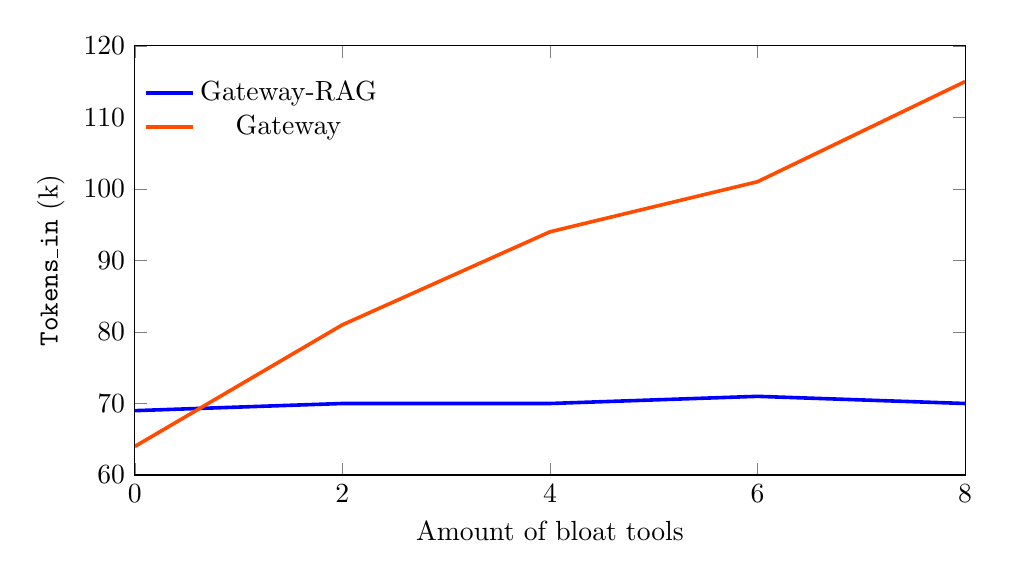
\begin{tikzpicture}
\begin{axis}[
  width=\linewidth,
  height=0.58\linewidth,
  xlabel={Amount of bloat tools},
  ylabel={\texttt{Tokens\_in} (k)},
  xmin=0, xmax=8,
  xtick={0,2,4,6,8},
  ymin=60, ymax=120,
  ytick={60,70,80,90,100,110,120},
  legend style={at={(0,0.85)},anchor=west,draw=none},
]
\addplot[line width=1.3pt,color=blue] coordinates {(0,69) (2,70) (4,70) (6,71) (8,70)};
\addplot[line width=1.3pt,color=red!70!yellow] coordinates {(0,64) (2,81) (4,94) (6,101) (8,115)};
\legend{Gateway-RAG, Gateway}
\end{axis}
\end{tikzpicture}
\caption{\texttt{Tokens\_in} under increasing capability load. Values are in thousands of tokens (k); the y-axis is truncated (60--120k) for readability.}
\label{fig:tokens_in_bloat}
\end{figure}
